%% fig1_model_schematic.tex -- standalone TikZ source for Figure 1 of
%% "Sparse data limit what a mechanistic corrosion model can predict".
%%
%% (a) the duplex scale, with the four boundary-moving reactions marked at the
%%     interface where each acts and the lattice-conservative ones in grey, and
%%     both state variables dimensioned in the SI coordinate convention
%%     (x = L_bl at m/bl, x = 0 at bl/ol, x = -L_ol at ol/water);
%% (b) the potential profile, drawn so that V = phi_m/bl + eps_f L_bl + phi_bl/e
%%     is visible as two interfacial steps and one constant-field ramp.
%%
%% Build:  pdflatex fig1_model_schematic.tex
%% (scripts/make_paper_figs.py also rasterizes it to .png)

\documentclass[tikz,border=6pt]{standalone}
\usepackage{amsmath,amssymb}
\usepackage{helvet}
\renewcommand{\familydefault}{\sfdefault}
\usepackage{sansmath}
\usetikzlibrary{arrows.meta,positioning,calc,fit,decorations.pathreplacing,backgrounds}

%% shared horizontal geometry: both panels use these x coordinates
\def\xL{0.60}      % left edge
\def\xNi{4.55}     % metal | Ni zone
\def\xMBL{5.55}    % Ni zone | barrier layer   (the m/bl interface, x = L_bl)
\def\xBLOL{10.55}  % barrier layer | outer layer (x = 0)
\def\xOLE{14.85}   % outer layer | water        (x = -L_ol)
\def\xR{18.75}     % right edge

\begin{document}\sansmath
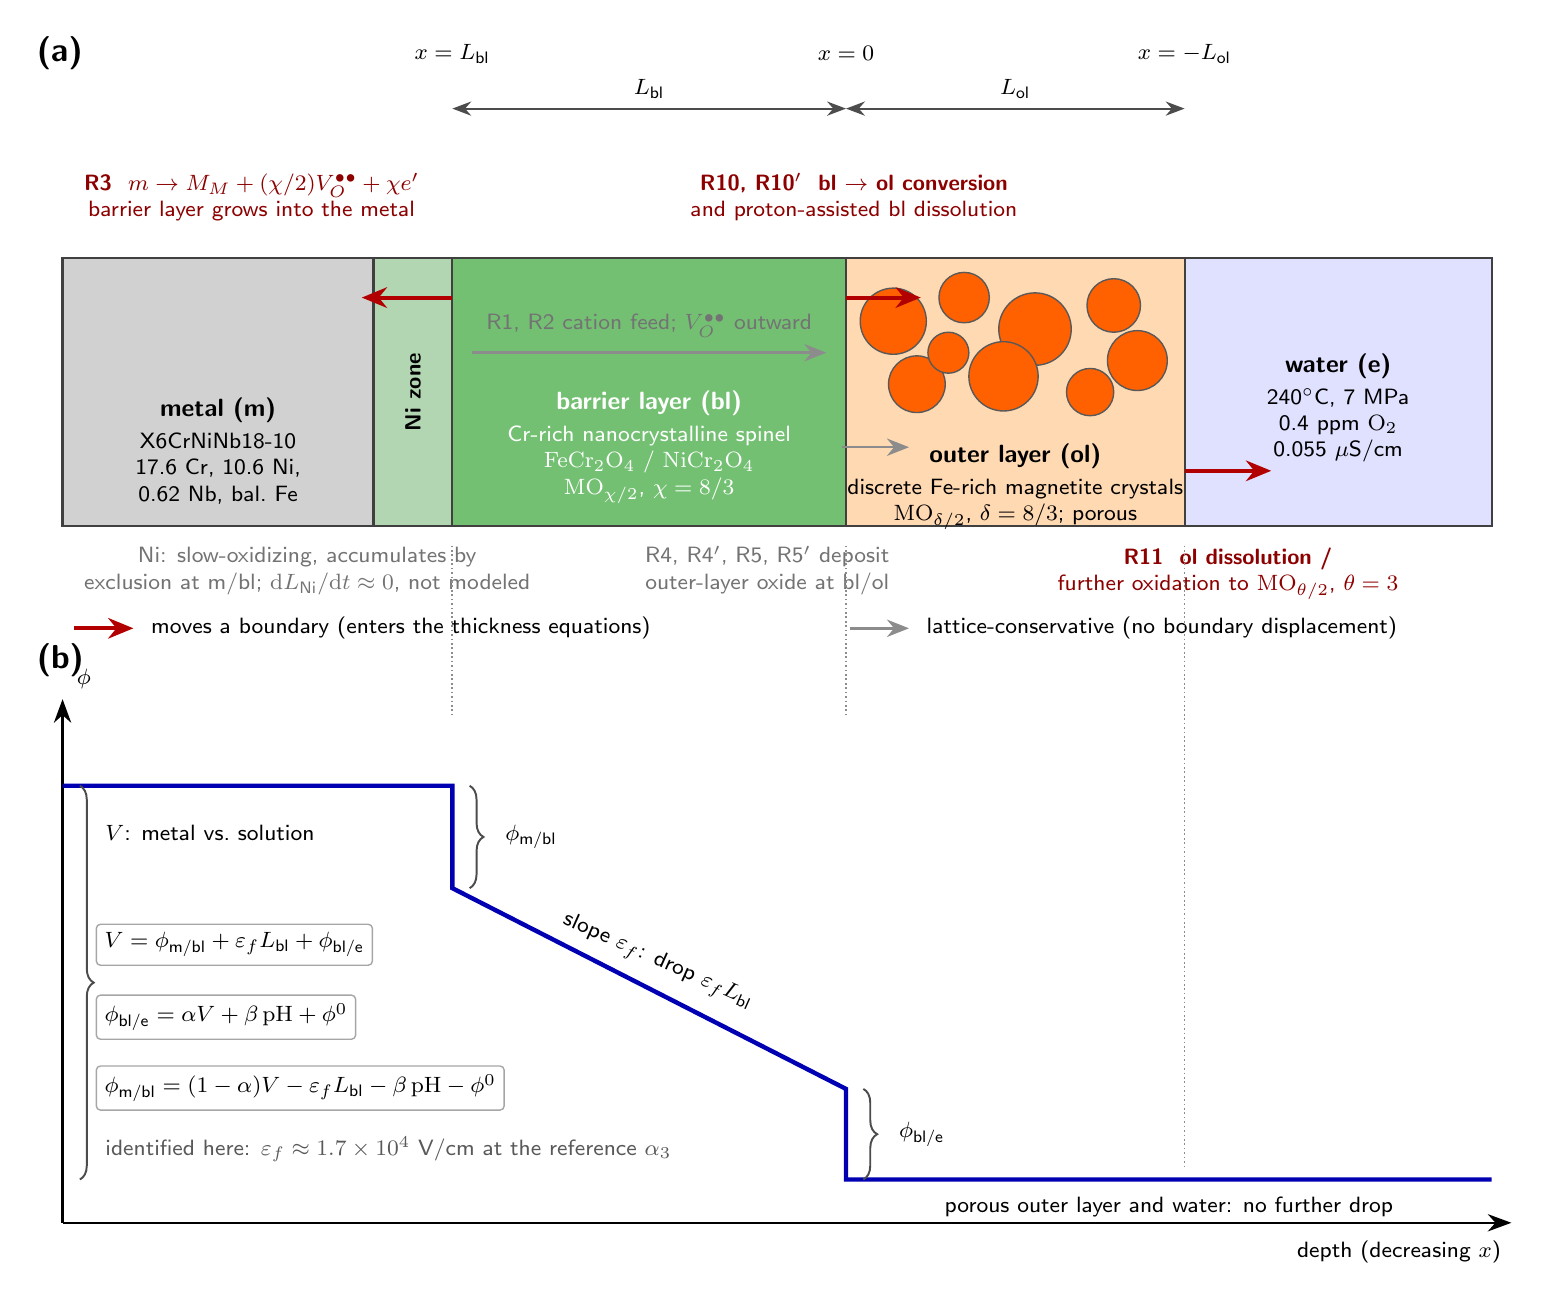
\begin{tikzpicture}[
  font=\sffamily\small,
  >={Stealth[length=3.0mm,width=2.2mm]},
  band/.style={draw=black!75,line width=0.8pt},
  rxn/.style={-{Stealth[length=3.2mm,width=2.6mm]},line width=1.5pt,draw=red!70!black},
  cons/.style={-{Stealth[length=2.8mm,width=2.2mm]},line width=0.9pt,draw=black!45},
  rlab/.style={font=\sffamily\footnotesize,align=center,text=red!55!black},
  clab/.style={font=\sffamily\footnotesize,align=center,text=black!55},
  dim/.style={{Stealth[length=2.4mm]}-{Stealth[length=2.4mm]},line width=0.7pt,draw=black!70},
  guide/.style={densely dotted,draw=black!45,line width=0.6pt},
  pot/.style={line width=1.6pt,draw=blue!70!black},
  brace/.style={decorate,decoration={brace,amplitude=5pt},draw=black!70,line width=0.7pt},
  eq/.style={font=\sffamily\footnotesize,align=center,inner sep=3pt,
             fill=white,draw=black!35,rounded corners=1.5pt,line width=0.5pt},
]

%% ================================================================ panel (a)
\def\ya{10.35} \def\yb{13.75}

\fill[black!18] (\xL,\ya) rectangle (\xNi,\yb);
\fill[green!45!black!30] (\xNi,\ya) rectangle (\xMBL,\yb);
\fill[green!55!black!55] (\xMBL,\ya) rectangle (\xBLOL,\yb);
\fill[orange!30] (\xBLOL,\ya) rectangle (\xOLE,\yb);
\fill[blue!12] (\xOLE,\ya) rectangle (\xR,\yb);

%% discrete crystals inside the porous outer layer
\foreach \cx/\cy/\cr in {11.15/12.95/0.42, 12.05/13.25/0.32, 12.95/12.85/0.46,
                         13.95/13.15/0.34, 11.45/12.15/0.36, 12.55/12.25/0.44,
                         13.65/12.05/0.30, 14.25/12.45/0.38, 11.85/12.55/0.26}{
  \fill[orange!75!red,draw=black!65,line width=0.5pt] (\cx,\cy) circle (\cr);
}

\draw[band] (\xL,\ya) rectangle (\xR,\yb);
\foreach \xi in {\xNi,\xMBL,\xBLOL,\xOLE}{ \draw[band] (\xi,\ya) -- (\xi,\yb); }

\node[align=center,font=\sffamily\footnotesize] at ({(\xL+\xNi)/2},11.30)
  {\small\bfseries metal (m)\\[2pt] X6CrNiNb18-10\\ 17.6 Cr, 10.6 Ni,\\ 0.62 Nb, bal.\ Fe};
\node[rotate=90,font=\sffamily\footnotesize,align=center] at ({(\xNi+\xMBL)/2},12.05)
  {\bfseries Ni zone};
\node[align=center,font=\sffamily\footnotesize,text=white] at ({(\xMBL+\xBLOL)/2},11.35)
  {\small\bfseries barrier layer (bl)\\[2pt] Cr-rich nanocrystalline spinel\\
   $\mathrm{FeCr_2O_4}$ / $\mathrm{NiCr_2O_4}$\\
   $\mathrm{MO}_{\chi/2}$, $\chi=8/3$};
\node[align=center,font=\sffamily\footnotesize] at ({(\xBLOL+\xOLE)/2},10.85)
  {\small\bfseries outer layer (ol)\\[2pt] discrete Fe-rich magnetite crystals\\
   $\mathrm{MO}_{\delta/2}$, $\delta=8/3$; porous};
\node[align=center,font=\sffamily\footnotesize] at ({(\xOLE+\xR)/2},11.85)
  {\small\bfseries water (e)\\[2pt] 240$^\circ$C, 7~MPa\\ 0.4~ppm $\mathrm{O_2}$\\ 0.055~$\mu$S/cm};

%% ---- reactions: bold red = moves a boundary, grey = lattice-conservative
\draw[rxn] (\xMBL,13.25) -- ++(-1.15,0);
\node[rlab,anchor=south west] at (\xL+0.15,14.10)
  {\bfseries R3\ \ $m \rightarrow M_M + (\chi/2)V_O^{\bullet\bullet} + \chi e'$\\
   barrier layer grows into the metal};

\draw[cons] (\xMBL+0.25,12.55) -- (\xBLOL-0.25,12.55);
\node[clab,anchor=south] at ({(\xMBL+\xBLOL)/2},12.62)
  {R1, R2 cation feed; $V_O^{\bullet\bullet}$ outward};

\draw[rxn] (\xBLOL,13.25) -- ++(0.95,0);
\node[rlab,anchor=south] at (\xBLOL+0.1,14.10)
  {\bfseries R10, R10$'$\ \ bl $\rightarrow$ ol conversion\\ and proton-assisted bl dissolution};

\draw[rxn] (\xOLE,11.05) -- ++(1.10,0);
\node[rlab,anchor=north,align=center] at (\xOLE+0.55,10.20)
  {\bfseries R11\ \ ol dissolution /\\ further oxidation to $\mathrm{MO}_{\theta/2}$, $\theta=3$};

\draw[cons] (\xBLOL-0.05,11.35) -- ++(0.85,0);
\node[clab,anchor=north] at (9.55,10.22)
  {R4, R4$'$, R5, R5$'$ deposit\\ outer-layer oxide at bl/ol};
\node[clab,anchor=north west] at (\xL+0.15,10.20)
  {Ni: slow-oxidizing, accumulates by\\ exclusion at m/bl; $\mathrm{d}L_\text{Ni}/\mathrm{d}t\approx0$, not modeled};

%% ---- thicknesses and the SI coordinate convention
\draw[dim] (\xMBL,15.65) -- node[above,font=\sffamily\footnotesize]{$L_\text{bl}$} (\xBLOL,15.65);
\draw[dim] (\xBLOL,15.65) -- node[above,font=\sffamily\footnotesize]{$L_\text{ol}$} (\xOLE,15.65);
\node[font=\sffamily\footnotesize] at (\xMBL,16.35) {$x=L_\text{bl}$};
\node[font=\sffamily\footnotesize] at (\xBLOL,16.35) {$x=0$};
\node[font=\sffamily\footnotesize] at (\xOLE,16.35) {$x=-L_\text{ol}$};

\node[font=\sffamily\bfseries\large,anchor=west] at (\xL-0.45,16.35) {(a)};

%% legend
\draw[rxn] (\xL+0.15,9.05) -- ++(0.75,0);
\node[anchor=west,font=\sffamily\footnotesize] at (\xL+1.00,9.05)
  {moves a boundary (enters the thickness equations)};
\draw[cons] (10.60,9.05) -- ++(0.75,0);
\node[anchor=west,font=\sffamily\footnotesize] at (11.45,9.05)
  {lattice-conservative (no boundary displacement)};

%% ================================================================ panel (b)
\def\ybase{2.05} \def\ymet{7.05} \def\ystep{5.75} \def\yramp{3.20}

\foreach \xi in {\xMBL,\xBLOL}{ \draw[guide] (\xi,\ya-0.25) -- (\xi,7.95); }
\draw[guide] (\xOLE,\ya-0.25) -- (\xOLE,\ybase+0.15);

\draw[->,line width=0.8pt] (\xL,\ybase-0.55) -- (\xR+0.25,\ybase-0.55)
  node[below left=1mm and 0mm,font=\sffamily\footnotesize]{depth (decreasing $x$)};
\draw[->,line width=0.8pt] (\xL,\ybase-0.55) -- (\xL,8.15)
  node[above right=0mm and 0.5mm,font=\sffamily\footnotesize]{$\phi$};

\draw[pot] (\xL,\ymet) -- (\xMBL,\ymet) -- (\xMBL,\ystep)
  -- (\xBLOL,\yramp) -- (\xBLOL,\ybase) -- (\xR,\ybase);

%% total potential difference
\draw[brace] (\xL+0.22,\ymet) -- (\xL+0.22,\ybase);
\node[anchor=west,font=\sffamily\footnotesize,align=left] at (\xL+0.42,6.45)
  {$V$: metal vs.\ solution};

%% the three contributions
\draw[brace] (\xMBL+0.22,\ymet) -- (\xMBL+0.22,\ystep);
\node[anchor=west,font=\sffamily\footnotesize] at (\xMBL+0.55,{(\ymet+\ystep)/2})
  {$\phi_\text{m/bl}$};
\draw[brace] (\xBLOL+0.22,\yramp) -- (\xBLOL+0.22,\ybase);
\node[anchor=west,font=\sffamily\footnotesize] at (\xBLOL+0.55,{(\yramp+\ybase)/2})
  {$\phi_\text{bl/e}$};
\node[anchor=south,font=\sffamily\footnotesize,align=center,rotate=-24]
  at ({(\xMBL+\xBLOL)/2},{(\ystep+\yramp)/2+0.10})
  {slope $\varepsilon_f$: drop $\varepsilon_f L_\text{bl}$};

\node[anchor=north,font=\sffamily\footnotesize,align=center] at ({(\xBLOL+\xR)/2},\ybase-0.10)
  {porous outer layer and water: no further drop};

\node[eq,anchor=north west] (eqv) at (\xL+0.42,5.30)
  {$V=\phi_\text{m/bl}+\varepsilon_f L_\text{bl}+\phi_\text{bl/e}$};
\node[eq,anchor=north west] (eq1) at (\xL+0.42,4.40)
  {$\phi_\text{bl/e}=\alpha V+\beta\,\mathrm{pH}+\phi^0$};
\node[eq,anchor=north west] (eq2) at (\xL+0.42,3.50)
  {$\phi_\text{m/bl}=(1-\alpha)V-\varepsilon_f L_\text{bl}-\beta\,\mathrm{pH}-\phi^0$};
\node[anchor=north west,font=\sffamily\footnotesize,text=black!65] at (\xL+0.42,2.72)
  {identified here: $\varepsilon_f\approx1.7\times10^{4}$~V/cm at the reference $\alpha_3$};

\node[font=\sffamily\bfseries\large,anchor=west] at (\xL-0.45,8.65) {(b)};

\end{tikzpicture}
\end{document}
